\cotefile{58}
\scanpage{52}
donc en les pts fermés $z'$ de $\overline{x'_1}\cap U$, on aurait $\operatorname{prof}F'_{z'}\leq 1$, ce qui est absurde. Donc si $i:U\to X'$ est l'inclusion, $F'_1=i_*(F'|U)$ est cohérent, et \unsure{évidemment|évidemt} de $\operatorname{prof}\geq 2$ en $X'-U$, d'autre part il est de $\operatorname{prof}\geq 2$ aux pts fermés de $\deleted{\unsure{X'|X}}U$, donc $F'_1$ est de $\operatorname{prof}\geq 2$ en \uline{tt} pt fermé de $X'$, on a gagné.
% archive sheet number: 51
\scanpage{53}\mspage{- 133 -}
\hfill n\textsuperscript{o} 371

$n-2$ \uline{de} $\underline{X}$ \uline{obtenu en supprimant dans} $\underline{X}$ \uline{les lignes d'indices} $i$ \uline{et} $j$ \uline{et les colonnes d'indices} $h$ \uline{et} $k$ ; \uline{on a alors}
\[
\csname tagsleft@true\endcsname
X^{ih}X^{jk}-X^{ik}X^{jh}=(\det\underline{X}).X^{ij,hk}.\tag*{(38)}
\]
Il suffit d'appliquer la formule (35) lorsque $H=I-\{i,j\}$, $K=I-\{h,k\}$, où $I=[\![1,n]\!]$.

Nous verrons au chap.IV que les formules (34) à (38) sont encore valables sans aucune hypothèse sur la matrice carrée $\underline{X}$.

\begin{center}
-:-:-:-:-
\end{center}
% archive sheet number: 52
\scanpage{54}
\begin{flushright}
Applications aux morphismes \uline{\deleted{\unsure{Lefschetz|hyperplans}} projectifs} et aux morphismes propres
\end{flushright}
% archive sheet number: 53
\scanpage{56}
\diagram{\begin{tikzcd}[ampersand replacement=\&,column sep=small,row sep=small]
Y\arrow[dr,bend right=24] \& {\subset P_k^r=X} \& {} \& {}\\
{} \& \text{section hyperplane,} \& U\ \text{voisinage de }Y, \& Z=X-U\\
{} \& \text{$F$ cohérent sur $X$} \& {} \& \text{ens fermé fini}
\end{tikzcd}}

a) Conditions pour que $H^i(U,F(-m))=0$ pour $m$ grand ?

a$'$) Condition pour que $\coprod_m H^i(U,F(m))$ de type fini sur $S$

b) Condition pour que $H^i(U,F(m))=0$ pour $m$ grd
\[
(i>0\text{ donné})
\]

\unsure{c|d}) Condition pour que
\[
H^i(U,F)\mathrel{\unsure{-|\to}}H^i(\widehat X,\widehat F)
\]
soit un isomorphisme ?

\textcircled{\scriptsize 1\textsuperscript{o}} Considérons la suite exacte \unsure{$C\colon$|($\colon$|(où} $E^{\unsure{d|j}}=\underline{\mathcal{E}xt}^{d}_{\underline O_X}(F,\omega_X)$

\diagram{\scriptsize\begin{tikzcd}[ampersand replacement=\&,column sep=1.0em,row sep=small]
{H^i_Z(X,F(-m))}\arrow[r,"\alpha_i"] \& {H^i(X,F(-m))}\arrow[r] \& {H^i(U,F(-m))}\arrow[r] \& {H^{i+1}_Z(X,F(-m))}\arrow[r,"\alpha_{i+1}",dash] \& {H^{i+1}(X,F(-m))}\\
{\displaystyle\prod_{z\in Z}E^{r-i}_{\unsure{e|\ell|z}}(m)^{\wedge}_{z}} \& {\Gamma E^{r-i}(m)}\arrow[l] \& {} \& {\displaystyle\prod_{z\in Z}E^{r-i-1}(m)^{\wedge}_{z}} \& {\Gamma E^{r-i-1}(m)}\arrow[l]
\end{tikzcd}}

Conditions équivalentes
\[
\left\{\begin{aligned}
&\Updownarrow\ \alpha_i\ \deleted{\unsure{sur|s}}\text{injectif pour }m\text{ grand}\quad\deleted{\unsure{[\text{ou, pour tt }m]}}\\
&z\in Z\ \Rightarrow\ z\text{ isolé dans }(\operatorname{Supp} E^{r-i}\cup\{z\})\\
&\unsure{\Leftrightarrow}\ \Updownarrow
\inserted{H^{i-1}(X,F(-m))\to H^{i-1}(U,F(-m))\ \text{\uline{surjectif} pour }m\text{ grand}}
\end{aligned}\right.
\]
\[
*\quad\left\{\begin{aligned}
&\alpha_i\text{ injectif pour }m\text{ grand, }i\leq n\quad\deleted{\Rightarrow}\\
&\Updownarrow\\
&\exists\ \text{voisinage ouvert }V\text{ de }Z,\text{ tel que }F\text{ soit de profondeur }>n\text{ sur }U\cap V\\
&\Updownarrow\\
&H^i(X,F(-m))\mathrel{\unsure{-|\to}}H^i(U,F(-m))\ \text{surjectif pour }m\text{ grand, }i<n
\end{aligned}\right.
\]
% archive sheet number: 55
\scanpage{57}
$F_{\unsure{o|0}}$ le Module qu'il induit sur $X_o$. On suppose \quad a) Pour tout $s\quad S$, la section $t_s$ induite par $t$ sur la fibre $X_s$ est $\underline{O}_{X_s}$-régulière et $\underline{F}_s$-régulière \quad b) $\underline{F}$ et $\underline{O}_X$ sont plats par rapport à $S$ \quad c) Pour tout $s\quad S$, $F_{o\ s}$, \deleted{et} $\underline{O}_{X_{o\ s}}$ \inserted{et $\underline{O}_{X_s}$} sont de profondeur $\quad 2$ en les points fermés de $X_{\deleted{\unsure{o|0}}s\ \deleted{s}}$. Sous ces conditions, il existe un Module cohérent $F$ sur $X$, et un isomorphisme de son complété formel $\widehat{F}$ le long de $X_o$ avec $\underline F$.

Cet énoncé va résulter du suivant:

\uline{Corollaire} 3.2. \quad Sous les conditions de 3\unsure{;|.}1. \quad (

\[
\handwritten{\coprod_{\substack{p\geq\unsure{p|0|p_0}\\ q\geq0}}F_0(q-p)}
\]
\[
\handwritten{M+M(1)+\text{- -}+M(-p)}
\qquad
\handwritten{\coprod_{0,q}S_q}
\]
\figure{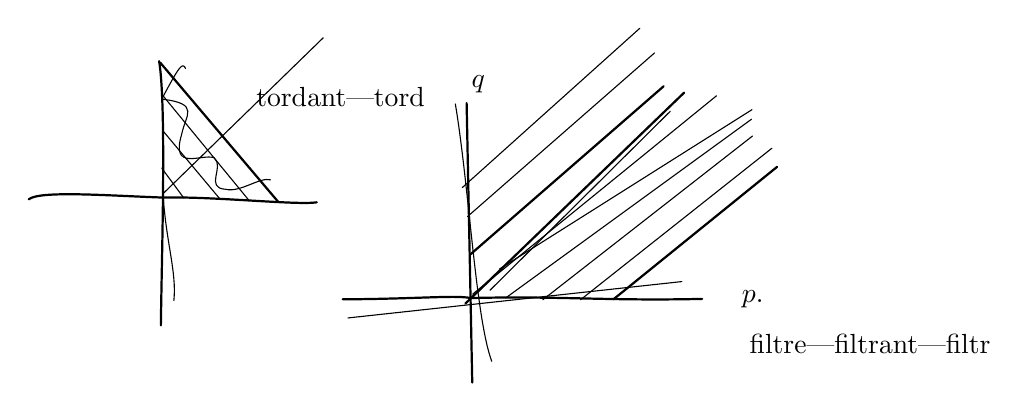
\begin{tikzpicture}[x=.55cm,y=.55cm,line cap=round,line join=round]
\draw[thick] (-3.1,-.04) .. controls (-2.85,.17) and (-1.2,.04) .. (0,0) .. controls (1.15,.03) and (3.1,-.18) .. (3.55,-.11);
\draw[thick] (-.09,3.15) .. controls (.08,2.1) and (-.03,-1.3) .. (-.05,-2.95);
\draw (0,.1) .. controls (.06,-1) and (.32,-1.72) .. (.25,-2.38);
\draw (-.03,.68)--(.48,-.01);
\draw (-.01,1.55)--(1.32,-.04);
\draw (0,2.35)--(1.98,-.06);
\draw[thick] (-.06,3.11)--(2.66,-.10);
\draw[thin] (0,.09)--(3.7,3.69);
\draw (0,2.33) .. controls (.37,3.02) and (.45,3.14) .. (.52,2.98);
\draw (0,2.27) .. controls (.86,2.16) and (.52,1.91) .. (.43,1.46) .. controls (.17,.59) and (.89,1.02) .. (1.18,.92) .. controls (1.43,.71) and (.95,.22) .. (1.45,.19) .. controls (1.78,.11) and (2.24,.48) .. (2.48,.41);
\begin{scope}[shift={(7.1,-2.32)}]
\draw[thick] (-2.95,-.03) .. controls (-1.2,-.02) and (-.35,.07) .. (0,0) .. controls (2.1,.05) and (3.15,-.07) .. (5.35,-.02);
\draw[thick] (-.09,4.5)--(.04,-1.95);
\draw[thin] (-.35,4.48) .. controls (-.03,2.55) and (.12,-.47) .. (.49,-1.46);
\draw[thin] (-2.83,-.46)--(4.88,.38);
\draw (-.19,2.55)--(3.91,6.23);
\draw (-.07,1.88)--(4.25,5.66);
\draw[thick] (0,1.01)--(4.46,4.89);
\draw[thick] (-.12,-.13)--(4.93,4.74);
\draw[thin] (.45,.18)--(4.61,4.31);
\draw (.05,.09)--(5.68,4.67);
\draw[thin] (.67,.67)--(6.5,4.35);
\draw (.81,0)--(6.49,4.13);
\draw (1.67,-.04)--(6.51,3.74);
\draw (2.54,-.04)--(6.96,3.46);
\draw[thick] (3.3,-.03)--(7.08,3.03);
\node[above] at (.18,4.51) {$\handwritten{q}$};
\node[left] at (-.83,4.64) {\handwritten{\unsure{tordant|tord}}};
\node[right] at (6.04,-.02) {\handwritten{$p$.}};
\node[right] at (6.22,-1.07) {\handwritten{\unsure{filtre|filtrant|filtr}}};
\end{scope}
\end{tikzpicture}}
\[
\handwritten{\mathscr F(n)}\qquad\handwritten{\mathscr F(n)}
\]
\[
\handwritten{H^i(X,F)\to H^i(\widehat X,\widehat F)}
\]
% archive sheet number: 56
\scanpage{58}
\[
\left\{\begin{aligned}
&\alpha_i\text{ bijectif pour }m\text{ grand}\\
&\Updownarrow\\
&\deleted{\unsure{E}}\operatorname{Supp} E^{r-i}\subset Z\\
&\Downarrow\\
&H^i_x(F_x)=0\quad\text{pour tt }x\text{ fermé \uline{dans $U$}.}
\end{aligned}\right.
\]
\[
\left\{\begin{aligned}
&\alpha_i\text{ bijectif pour }m\text{ grd, }\ i\leq n\\
&\Updownarrow\\
&\operatorname{supp}E^{r-i}\subset Z\quad\text{pour }i\leq n\\
&\Updownarrow\\
&\operatorname{prof}(F_x)>n\quad\text{pour tt }x\text{ fermé \uline{dans} }U\\
&\Updownarrow\\
&H^i(U,F(-m))=\deleted{H^i(\unsure{X|U},F(-m))\ \text{bijectif pour }i\unsure{<|\leq}n}
\inserted{0\ \text{pour }m\text{ grand, }i<n\text{ \uuline{et}}}\\
&H^n(U,F(-m))\to H^{n+1}_Z(X,F(-m))
\deleted{\text{\unsure{injectif|surjectif} pour }i\leq\unsure{n|i+1}}\ \inserted{\text{injectif}}
\end{aligned}\right.
\]
\margin{\textcircled{$B_n$}}
\[
\left\{\begin{aligned}
&\alpha_i\text{ bijectif pour }m\text{ grd, }\ i\leq n\\
&\qquad\text{et }\alpha_i\text{ injectif pour }m\text{ grd, }\ i=n+1\\
&\Updownarrow\\
&\deleted{\operatorname{prof}}\operatorname{Supp} E^{r-i}\subset Z\quad\text{pour }i\leq n,\quad
\operatorname{supp} E^{r-n-1}\text{ ne peut}\\
&\qquad\text{avoir un pt de }Z\text{ que comme pt isolé}\\
&\Updownarrow\\
&\operatorname{prof}(F_x)>n\quad\text{si }x\text{ fermé dans }U,\quad\text{et}\\
&\operatorname{prof}(F_x)>n+1\quad\text{si de plus }x\in V\cap U,\ V\text{ voisinage}\\
&\qquad\text{ouvert convenable de }Z\\
&\Updownarrow\\
&H^i(U,F(-m))=0\quad\text{pour }m\text{ grd, }\ i\leq n\\
&\Updownarrow\\
&\coprod_{m\geq0} H^i(U,F(-m))\ \text{de type fini sur }S(-h)\ \text{et pr }i\leq n
\end{aligned}\right.
\]
% slanted
\margin{$H^i(U,F)$ de dim finie pour $i\leq n$ $\overset{\text{cf }2^{\mathrm o}}{\Longleftarrow}$}
Cela résout la question (a). Sous les conditions de $(*)$, on a donc [si $t$ est $F$-régulier]
\[
\left\{\begin{aligned}
&H^i(U,F)\xrightarrow{\sim} H^i(\widehat X,\widehat F)\quad\text{est }
\begin{cases}\text{iso si }i<n\\ \text{mono si }i=n\end{cases}\\
&H^i(\widehat X,\widehat F)\xrightarrow{\sim}\varprojlim H^i(X_m,F_m)\quad\text{pour }i\leq n
\end{aligned}\right.
\]
% archive sheet number: 57
\scanpage{59}
Ce qui donne des conditions suffisantes pour la validité de c). Cependant, elles ne sont pas nécessaires [\unsure{$=$|$\bar m$} en exigeant la validité de c pour $i<n$, et tous les tordus de $F$], comme on voit en faisant $n=1$ : alors il suffit qu'on ait $\operatorname{prof} F_x\geq2$ pour $x$ fermé dans $U$, pour pouvoir conclure que
\[
H^0(U,F)\mathrel{\unsure{-|\to}}H^0(\widehat X,\widehat F)
\]
est bijectif.

\textcircled{\scriptsize 2\textsuperscript{o}} La suite exacte nous apprend que \unsure{l'ar.|l'hom.|l'homom.} $H^i(U,F)\to H^{i+1}_Z(X,F)$ est un isom mod vectoriels finis. Donc
\[
\deleted{H^i(U,F}
\]
\margin{\textcircled{$A'_i$}}
\[
\left\{\begin{aligned}
&H^i(U,F)\text{ de dim finie sur }k\\
&\Updownarrow\\
&H^{i+1}_z(F_z)\text{. de dim finie [i.e. de \unsure{long.|lg.} finie] pour tt }z\in Z\\
&\Updownarrow\\
&z\deleted{\unsure{\notin|\subset}}\in Z\ \Longrightarrow\ z\text{ pt isolé de }\operatorname{supp} E^{r-i-1}\cup\{z\}\\
&\Updownarrow\\
&\alpha_{i+1}\text{ injectif pour }m\text{ grand}\\
&\Updownarrow\\
&H^i(X,F(-m))\mathrel{\unsure{-|\to}}H^i(\deleted{X}U,F(-m))\ \text{surjectif pour }m\text{ grand}
\end{aligned}\right.
\]
% archive sheet number: 58
\scanpage{60}
\[
R^p f_*\bigl[R^{\unsure{q|1}} g_*(F)\bigr]\deleted{\unsure{f(m)|({m})}})
\]
\deleted{\[
H^i(U,F(m))\to H^i_{Y}
\]
\[
H^i(U,F(m))
\]
\[
\Updownarrow
\]
3\textsuperscript{o})
\[
\begin{aligned}
&\coprod_{m\geq0}H^i(U,F(m))\quad\text{de type fini sur }S\\
&\hspace{9em}\text{pour }i\leq n\\
&\Updownarrow\\
&R^i g_*(F)\text{ coh. pour }i\leq n,\ \text{i.e. }\underline H^i_Z(F)\text{ coh pr }i\leq n+1\\
&\quad\text{\uline{i.e. $H^i_z(F_z)$ de dim finie pour $i\leq n+1$}},z\in Z
\end{aligned}
\]}
\margin{\textcircled{$A^{\unsure{\prime|f}}_n$}}
\[
\left\{\begin{aligned}
&H^i(U,F)\text{ de dim finie si }i\leq n\\
&\Updownarrow\\
&F\text{ de prof }>n+1\quad\text{sur }U\text{ au voisinage de }Z\\
&\Updownarrow\\
&z\in Z\ \Longrightarrow\ z\text{ pt isolé de }\operatorname{supp}E^{r-i-1}\cup\{z\}\quad\text{si }i\leq n\\
&\Updownarrow\\
&\alpha_i\text{ injectif pour \uline{\unsure{très|$m$} grand} si }i\leq n+1\\
&\Updownarrow\\
&H^i(X,F(-m))\mathrel{\unsure{-|\to}}H^i(U,F^{\unsure{\prime|\vee}}(-m))\quad\text{surjectif pr }m\text{ grd, }i\leq n\\
&\Updownarrow\\
&R^ig_*(F)\text{ coh. pour }i\leq n,\quad\Longleftrightarrow H^i_z(F)\text{ de dim finie}\\
&\hspace{16em}\text{pour }z\in Z,\ i\leq n+1\\
&\Updownarrow\\
&\coprod_{\text{\textcircled{\scriptsize $m\geq0$}}}H^i(U,F(m))\quad\text{de type fini sur }S\quad\text{pr }i\leq n
\end{aligned}\right.
\]
% archive sheet number: 59
\scanpage{61}
$F_{\unsure{o|0}}$ le Module qu'il induit sur $X_o$. On suppose \quad a) Pour tout $s\quad S$, la section $t_s$ induite par $t$ sur la fibre $X_s$ est $\underline O_{X_s}$-régulière et $\underline F_s$-régulière \quad b) $\underline F$ et $\underline O_X$ sont plats par rapport à $S$ \quad c) Pour tout $s\quad S$, $F_{o\ s}$, \deleted{et} $\underline O_{X_{o\ s}}$ \inserted{et $\underline O_{X_s}$} sont de profondeur $\quad2$ en les points fermés de $X_{\deleted{\unsure{o|0}}s\ \deleted{s}}$. Sous ces conditions, il existe un Module cohérent $F$ sur $X$, et un isomorphisme de son complété formel $\widehat F$ le long de $X_o$ avec $\underline F$.

Cet énoncé va résulter du suivant:

\uline{Corollaire} 3.2. \quad Sous les conditions de 3;1. \quad (

\[
\handwritten{\sum_{p\geq0}R^i f_{0*}F_0(q-p)\qquad q-p\geq m}
\]
\[
\handwritten{S_{\unsure{pq|M}}=
\begin{cases}
0&\text{si }p>0\\
\unsure{Sq|S_q}&\text{si }p=0
\end{cases}}
\]
\figure{\begin{tikzpicture}[x=.67cm,y=.67cm,line cap=round,line join=round]
\draw[thin] (-.01,-1.04) .. controls (.08,.62) and (-.16,2.8) .. (-.14,4.31);
\draw[very thin] (-.18,.02)--(-.24,4.10);
\draw[thin] (-.76,.05) .. controls (1.53,.20) and (4.42,.11) .. (6.03,.08);
\draw[very thin] (-.71,-.02)--(-.83,.04)--(-.61,.10);
\draw[thick] (-.02,.05)--(-.04,-.18) .. controls (1.04,-.02) and (3.15,.04) .. (4.67,-.14) .. controls (5.32,-.21) and (5.96,-.30) .. (6.03,-.19) -- (6.01,.18);
\draw[thin] (5.33,-.03)--(5.95,-.09);
\draw[very thin,gray] (.04,.64)--(5.42,.78);
\node[above left] at (-.48,4.04) {$\handwritten{q}$};
\node[right] at (6.04,-.03) {$\handwritten{p}$};
\node at (4.94,3.90) {$\handwritten{F_0(-p)}$};
\begin{scope}[shift={(8.9,-.12)}]
\draw[thin] (0,4.24) .. controls (.22,2.77) and (.04,.79) .. (.10,-1.30);
\draw[thin] (.24,-1.11)--(.09,-2.68);
\draw[thin] (-.9,.10) .. controls (.62,-.06) and (3.1,.15) .. (5.42,.00);
\draw[very thin,gray] (-.95,-3.56)--(6.12,1.89);
\end{scope}
\end{tikzpicture}}
% archive sheet number: 60
\scanpage{62}
\[
C'_i\ \left\{\begin{aligned}
&H^i(U,F(m))=0\quad\text{pour }m\text{ grand}\quad(i>0\text{ donné})\\
&\Updownarrow\\
&\underline H^{i+1}_Z(F)=0\quad\text{i.e.}\quad H^{i+1}_z(F_{\unsure{z|c}})=0\quad\text{pr }z\in Z\\
&\Updownarrow\\
&R^i g_*(F)=0
\end{aligned}\right.
\]
\[
\deleted{\unsure{\Updownarrow|\Downarrow}}\Downarrow
\]
\[
C_n\ \left\{\begin{aligned}
&H^i(U,F(m))=0\quad\text{pr }m\text{ grd,}\qquad0<i\leq n\\
&\hspace{16em}(n\geq1\text{ donné})\\
&\Updownarrow\\
&\deleted{H^i}\ [\text{à supposer que } F=g_*(F|U)]\quad\operatorname{prof}_z F>n+1\\
&\hspace{16em}\text{pr }z\in Z
\end{aligned}\right.
\]
Les conditions $C$ sont les seules qui exigent quelque chose sur la profondeur en les $z\in Z=X-U$ ..... et non seulement aux pts de $U$.

\figure{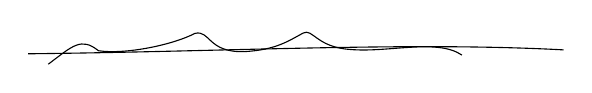
\begin{tikzpicture}[x=.85cm,y=.55cm]
\draw (0,0) .. controls (3,.05) and (5.7,.28) .. (8,.09);
\draw (.30,-.24) .. controls (.67,.19) and (.79,.39) .. (1.05,.07)
 .. controls (1.45,-.02) and (2.15,.20) .. (2.49,.47)
 .. controls (2.72,.56) and (2.68,.02) .. (3.23,.05)
 .. controls (3.70,.09) and (3.88,.29) .. (4.11,.48)
 .. controls (4.25,.59) and (4.31,.15) .. (4.81,.10)
 .. controls (5.38,.02) and (6.11,.36) .. (6.48,-.03);
\end{tikzpicture}}
% archive sheet number: 61
\scanpage{63}\mspage{- 7 -}
$(B_q)$. \uline{Il existe un sous-groupe invariant} $C$ \uline{de} $G$ \uline{qui est cyclique d'ordre premier à} $q$, \uline{et qui est tel que} $G/C$ \uline{soit un} $q$-\uline{groupe}.

Le résultat suivant est dû à Brauer [3] et Witt [18] :

PROPOSITION 2. \uline{Soit} $G$ \uline{un groupe fini et soit} $E$ \uline{un corps de caractéristique zéro}. \uline{Supposons que, pour tout nombre premier} $q$, \uline{et pour tout sous-groupe} $H$ \uline{de} $G$ \uline{vérifiant} $(B_q)$, \uline{l'algèbre} $E[H]$ \uline{soit décomposée}. \uline{Alors} $E[G]$ \uline{est décomposée}.

Rappelons brièvement la démonstration :

On commence par établir une formule :
\[
\csname tagsleft@true\endcsname
1=\mathop{\vphantom{\sum}}\limits_{\lambda}\ n_\lambda\varphi_\lambda^*,\qquad n_\lambda\in\text{\uuline{$Z$}},\tag*{(12)}
\]
où les $\varphi_\lambda$ sont des caractères de représentations rationnelles sur $E$ de sous-groupes $H_\lambda$ vérifiant $(B_{q_\lambda})$, et où $\varphi_\lambda^*$ désigne le caractère de $G$ \uline{induit} par $\varphi_\lambda$ ; voir Witt [18], Satz 6, ou bien Swan [14], th.4.1.

Si maintenant $\chi$ est un caractère de $G$ à valeurs dans $E$, on multiplie (12) par $\chi$, et l'on obtient :
\[
\csname tagsleft@true\endcsname
\chi=\handwritten{\sum}n_\lambda\varphi_\lambda\mathord{*}\chi
=\handwritten{\sum}n_\lambda(\varphi_\lambda\chi)\mathord{*}.\tag*{(13)}
\]
Comme $\varphi_\lambda\chi$ est un caractère de $H$ à valeurs dans $E$, l'hypothèse faite sur les $H_\lambda$ montre que c'est le caractère d'une représentation de $H_\lambda$ rationnelle sur $E$ ; donc $(\varphi_\lambda\chi)\mathord{*}$ est le caractère d'une représentation de $G$ rationnelle sur $E$. La formule (13), jointe au critère (b) ci-dessus, montre que $\chi$ est le caractère d'une représentation de $G$ rationnelle sur $E$. Ceci ayant lieu pour tout $\chi$, la prop.1 montre que $E[G]$ est décomposée, cqfd.

3. \uline{Démonstration du théorème 3}.

Compte tenu de la prop.1, il s'agit de prouver que, \uline{si} $G$ \uline{vérifie} $(R_p)$ \uline{et si} $\ell\ne p$, \uline{l'algèbre} $Q_\ell[G]$ \uline{est décomposée}. De plus, la prop.2 permet de supposer qu'il existe un nombre premier $q$ tel que $G$ vérifie $(B_q)$. Nous
% archive sheet number: 62
\scanpage{65}
\[
\underline O_{\widehat C}(1)\quad\rightsquigarrow\quad \underline O_{\widehat C_X}(1)
\]
\[
\widehat C=\operatorname{Spec} S[z]\qquad
\left\{\begin{aligned}&\text{induit }0\\&\text{sur }C\text{ et}\\&\text{sur }C'\end{aligned}\right.
\]
\[
\underline O_{\widehat C}(1)
\]
\diagram{\scriptsize\begin{tikzcd}[ampersand replacement=\&,column sep=large,row sep=2.8em]
\deleted{\operatorname{Pic} C} \& \operatorname{Pic}(\widehat C)\arrow[r] \& {} \& \unsure{\text{iso}|0}\\
\operatorname{Pic}(X)\arrow[u]\arrow[r,"{\text{injectif,}}","{\substack{\text{[bijectif}\\\text{dans le cas}\\X\ \text{\unsure{loc|\deleted{loc.}} factoriel]}}}"']\arrow[rr,bend left=31,"{\text{noyau \unsure{contient|contenu}}}"]
\& \operatorname{Pic}(\widehat C')\arrow[r]\arrow[dr] \& \operatorname{Pic}(C')\arrow[r,"{\substack{\text{injectif}\\\text{[surjectif}\\\text{dans le}\\\text{cas }\deleted{\unsure{\text{loc}|\text{loc.}}}\\\text{factoriel]}}}"'] \& \operatorname{Pic}(\widetilde C')\\
{} \& {} \& {\substack{\text{noyau}\\ \bigl[\text{engendré par}\\\text{l'image de }\underline O_X(1)}} \& {}
\end{tikzcd}}
\[
\operatorname{Pic}(X)/Z.\unsure{\xi|\zeta}\ \subset\ \operatorname{Pic}(\widehat C')/Z\xi)
\]
\margin{$\unsure{g/f|g/f^n|g/f^m}\qquad 1/g$}
\margin{$g^m=uf^n$\\ $\deleted{\unsure{g=v}}$\\ $\deleted{\unsure{g^m/f^n|g^m/f}}$\\ $g=uf^k$\\ $g^m/f^n=u$}
\margin{$\unsure{\varphi|g}^{n}$ est une unité donc $\varphi$ est une unité}

\[
\boxed{\operatorname{Pic}(C)=0\quad ??}
\]
\diagram{\scriptsize\begin{tikzcd}[ampersand replacement=\&,column sep=small,row sep=2.0em]
{} \& {} \& 0\arrow[d] \& {}\\
{} \& Z.\xi\arrow[r,equal]\arrow[d] \& Z\xi\arrow[d,"{\text{\textcircled{?}}}"] \& {}\\
\unsure{\bullet|0}\arrow[r] \& \operatorname{Pic}(X)\arrow[r,"{\substack{\text{injectif}\\\text{[surjectif]}}}"'] \& \operatorname{Pic}(\widehat C')\arrow[d,"{\substack{\deleted{\text{injectif}}\\\text{[surjectif]}}}"] \& {}\arrow[l]\\
{} \& \operatorname{Pic}(C)\arrow[r] \& \operatorname{Pic}(C')\arrow[r] \& \operatorname{Pic}(\widetilde C')
\end{tikzcd}}
\[
\boxed{\operatorname{Pic}(\unsure{\ell|C|A})=0\ ?}
\]
$\operatorname{Pic}$

\figure{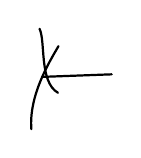
\begin{tikzpicture}[x=.65cm,y=.65cm,line cap=round]
\draw[thick] (-.17,.96) .. controls (-.05,.72) and (-.18,-.08) .. (.19,-.29);
\draw[thick] (-.33,-1.00) .. controls (-.38,-.34) and (.02,.31) .. (.20,.62);
\draw[thick] (-.12,.02)--(1.24,.07);
\end{tikzpicture}}
% archive sheet number: 64
\scanpage{66}
\[
X-a
\]
\diagram{\resizebox{\linewidth}{!}{\begin{tikzcd}[ampersand replacement=\&,column sep=.55em,row sep=.2em]
\bullet\arrow[r] \& H^0_{\unsure{a|-}}(X,\underline O_X^*)\arrow[r] \& H^0(X,\underline O_{\unsure{X|x}}^*)\arrow[r] \& H^0(U,\underline O_{\unsure{U|X}}^*)\arrow[r] \& H^{\unsure{1}}_a(X,O_X^*)\arrow[r] \& H^1(X,\underline O_X^*)\arrow[r]\arrow[d,equal] \& H^1(U,O_X^*)\arrow[r] \& \underline{H^2_a(\unsure{X},\underline O_X^*)}\arrow[r] \& \underline{H^2(X,\underline O_X^*)}\\
{} \& {} \& {} \& {} \& {} \& 0 \& {} \& {} \& {}
\end{tikzcd}}}
\[
A^*\longrightarrow\widetilde A^*\qquad
\]
\[
\deleted{\unsure{a}}\qquad F\quad H^0_x(F)
\]
\figure{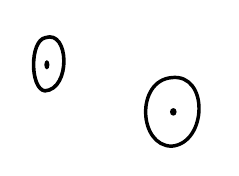
\begin{tikzpicture}[x=.65cm,y=.65cm,line cap=round]
\draw[line width=1.3pt] (0,.06) .. controls (-.29,.10) and (-.30,1.04) .. (.01,1.10) .. controls (.48,1.26) and (.51,.09) .. (0,.06);
\fill (.04,.57) ellipse (.05 and .09);
\draw[line width=1.25pt] (2.48,-1.02) .. controls (1.83,-1.02) and (1.77,.26) .. (2.48,.32) .. controls (3.21,.40) and (3.17,-.96) .. (2.48,-1.02);
\fill (2.51,-.35) ellipse (.065 and .075);
\end{tikzpicture}}
\diagram{\scriptsize\begin{tikzcd}[ampersand replacement=\&,column sep=1.2em,row sep=1em]
{} \& \text{loc. factoriel}\arrow[r,Rightarrow]\arrow[dr,Rightarrow] \& \text{\inserted{loc.} quasi-factoriel}\arrow[r,Rightarrow] \& \text{parafactoriel}\\
\widetilde A\longrightarrow\widetilde A_0 \& {} \& \text{1\unsure{-}factoriel,}\arrow[l]\arrow[d,Rightarrow] \& {}\\
\deleted{\unsure{\widetilde A=}} \& {} \& \text{0-factoriel,} \& {}
\end{tikzcd}}
\[
H^1(X,\underline O_X)=0
\]

$L\qquad L_B$
\figure{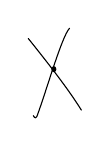
\begin{tikzpicture}[x=.50cm,y=.50cm,line cap=round]
\draw (-.65,.78) .. controls (-.20,.22) and (.36,-.49) .. (.70,-1.04);
\draw (.40,1.04) .. controls (.20,.83) and (-.19,-.56) .. (-.43,-1.20) .. controls (-.47,-1.29) and (-.52,-1.18) .. (-.52,-1.18);
\fill (0,0) ellipse (.065 and .078);
\end{tikzpicture}}
\[
\begin{matrix}\widetilde X\\[.4em]X\end{matrix}
\qquad
\begin{aligned}&\deleted{\unsure{1-d=|1-2=|1\ \text{dim}}}\\ &1-h^1=2-h'-h''\end{aligned}
\]
\[
J\subset A\subseteq B\qquad
\]
\[
\vdots\qquad \underline{A/J\qquad B/JB}
\]
\[
\begin{aligned}
1-g&=\sum(1-g_i)-\sum n_s\quad\unsure{=-}\\
1-g&=\unsure{\nu|v}-\sum g_i-\sum n_s
\end{aligned}
\]
\figure{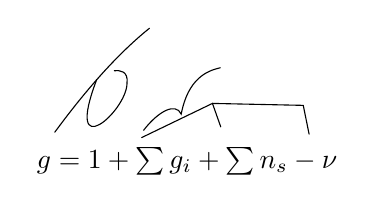
\begin{tikzpicture}[x=.62cm,y=.62cm,line cap=round]
\draw (-1.66,-.08) .. controls (-1.10,.68) and (-.44,1.47) .. (.28,2.05);
\draw (-.80,1.00) .. controls (-1.48,-.78) and (-.19,.34) .. (-.18,.92) .. controls (-.15,1.18) and (-.33,1.19) .. (-.44,1.18);
\draw (.16,-.04) .. controls (.46,.35) and (.82,.54) .. (.93,.29) .. controls (1.07,1.02) and (1.46,1.18) .. (1.73,1.24);
\draw (.12,-.19)--(1.57,.51)--(1.74,.03);
\draw (1.57,.51)--(3.43,.47)--(3.55,-.12);
\node[below] at (1.05,-.19) {$g=1+\sum g_i+\sum n_s-\nu$};
\end{tikzpicture}}
\figure{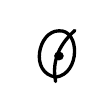
\begin{tikzpicture}[x=.47cm,y=.47cm,line cap=round]
\draw[very thick] (0,-.56) .. controls (-.72,-.46) and (-.49,.69) .. (.08,.69) .. controls (.65,.73) and (.66,-.47) .. (0,-.56);
\draw[very thick] (-.01,-.68) .. controls (-.13,-.08) and (.14,.37) .. (.51,.70);
\fill (.08,.01) ellipse (.13 and .12);
\end{tikzpicture}}
\[
\begin{array}{ll}
1-g=1-g'-\sum n_s & 1-g=2-g'-g''-\sum n_s\\[.6em]
g=g'+\sum n_s & g=(g'+g'')+\sum n_s-1
\end{array}
\]
\figure{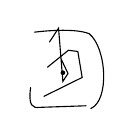
\begin{tikzpicture}[x=.50cm,y=.50cm,line cap=round]
\draw (-.88,1.00) .. controls (-.47,1.05) and (.19,1.09) .. (.51,.96) .. controls (.95,.60) and (1.03,-.73) .. (.55,-.94);
\draw (-.98,-.41) .. controls (-1.04,-.88) and (-.93,-.93) .. (-.75,-.91)--(.43,-.87);
\draw (-.64,-.63)--(.33,-.15)--(.22,.51)--(-.02,.54)--(-.55,.11);
\draw (-.50,.75)--(-.27,1.10)--(-.16,-.25)--(-.03,-.05)--(-.20,.31);
\fill (-.16,-.03) circle (.06);
\end{tikzpicture}}
\[
k[\unsure{x|u},y,z]/xy
\]
\figure{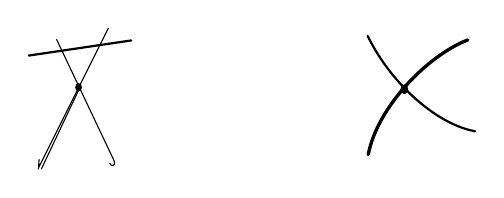
\begin{tikzpicture}[x=.62cm,y=.62cm,line cap=round]
\draw[thick] (-1.04,.67)--(1.06,.98);
\draw (-.47,1.00)--(.71,-1.49) .. controls (.74,-1.62) and (.64,-1.59) .. (.62,-1.54);
\draw (.59,1.23)--(-.84,-1.63)--(-.83,-1.46);
\draw (-.78,-1.65)--(-.02,-.04);
\fill (-.02,.02) ellipse (.07 and .085);
\begin{scope}[xshift=4.1cm]
\draw[thick] (-.71,1.07) .. controls (-.21,.05) and (.74,-.75) .. (1.49,-.88);
\draw[very thick] (-.70,-1.36) .. controls (-.51,-.37) and (.53,.68) .. (1.34,.99);
\fill (.04,-.02) ellipse (.08 and .10);
\end{scope}
\end{tikzpicture}}
\[
\deleted{g'+g''}\qquad g'=g''=0\qquad\sum g_i
\]
% archive sheet number: 65
\scanpage{67}
$X$ schéma projectif sur $k$, \qquad $\Gamma(X,\underline O_X)\simeq k$

$C$ son cône projetant affine, $a$ son sommet

$\widehat C$ \unsure{le|son} cône projetant projectif

\diagram{\begin{tikzcd}[ampersand replacement=\&,column sep=1.4em,row sep=2.8em]
X\arrow[r,"i",dash]\arrow[d] \& X'\arrow[r,"\pi"]\arrow[d,"f","{\substack{\text{\unsure{cartésien|section}}\\\text{par II}\\8.7.5.}}"'] \& X\\
a\arrow[r] \& \widehat C\arrow[r,dash] \& {}
\end{tikzcd}}

\deleted{$\operatorname{Pic}(X)\xrightarrow[\sim]{\pi^*}\operatorname{Pic}(X')$, et}
[car $X'$ est un fibré projectif sur $X$]

donc $\operatorname{Pic}(X')\mathrel{\overset{\unsure{4^o|\pi^*|\mathrm{ct}}}{\sim}}\operatorname{Pic}(X)\mathbin{x}Z$
\deleted{[\unsure{$\mathcal L$|la} \illegible{2} $\unsure{X}$]}

$i^*\colon\operatorname{Pic}(X')\mathrel{-}\operatorname{Pic}(X)$ a comme noyau $=Z$, engendré par $\underline O_{X'}(1)$

$\operatorname{Pic}(\widehat C)\longrightarrow\operatorname{Pic}(X')$ injectif
[car $f_*(\underline O_{X'})=\underline O_{\widehat C}$]

\unsure{Il s'ensuit|Je m'assure} que
\[
\boxed{\operatorname{Pic}(\widehat C)\unsure{\simeq|=}Z}
\boxed{\xrightarrow{\sim}\operatorname{Ker}\bigl[\operatorname{Pic}(X')\mathrel{\overset{i^*}{-}}\operatorname{Pic}(X)\bigr]}
\]
\hfill par \uline{II} 8.8.6.

Soit $C_X$ la partie de $X'$ au dessus de $C$, c'est un fibré \unsure{vectoriel|\deleted{vectoriel}} de \unsure{rang|\deleted{rang}} $1$ sur $X$.

Je dis que
\[
\operatorname{Pic}(X)\xrightarrow{\sim}\operatorname{Pic}(C_X)\qquad (?)
\]
% slanted
\margin{faut-il supposer $X$ localement factoriel ??}
Cet hom est \unsure{évidemment} injectif, car son composé avec $j^*\colon\operatorname{Pic}(C_X)\mathrel{-}\operatorname{Pic}(X)$, \inserted{est} \deleted{\unsure{l'injection}} \deleted{la section nulle de $C_X$ sur} l'identité. Pour la \uline{surjectivité}, on note que au dessus d'un ouvert convenable de $X$,
% archive sheet number: 66
